\documentclass[11pt,a4paper]{article}
\usepackage[margin=18mm,top=22mm,bottom=20mm]{geometry}
\usepackage{fontspec}\setmainfont{Latin Modern Roman}
\usepackage{xcolor}\usepackage{amsmath,amssymb,tikz,graphicx,fancyhdr,array,needspace}
\usetikzlibrary{patterns,arrows.meta,decorations.pathmorphing,calc}
\setlength{\headheight}{14pt}
\usetikzlibrary{arrows.meta}
\pagestyle{fancy}\fancyhf{}\renewcommand{\headrulewidth}{0.4pt}
\fancyhead[L]{\textbf{M-09}}\fancyhead[C]{\itshape Fizika — yechimlar (OliyFizika.uz)}\fancyhead[R]{\textbf{Mock №9}}
\fancyfoot[C]{\thepage}
\setlength{\parindent}{0pt}\setlength{\parskip}{3pt}
\newcommand{\opt}[2]{\hspace*{4mm}#1)\ #2\par}
\newcommand{\blank}{\rule{5cm}{0.4pt}}
\begin{document}

\begin{center}{\Large\textbf{FIZIKA — YECHIMLAR}}\\[2pt]{\large Mock №9}\end{center}
\Needspace{10\baselineskip}\noindent\begin{minipage}{\linewidth}
\textbf{1.}\ Massasi 2 t bölgan avtomobilni 0,5 m/s$^{2}$ tezlaniş bilan şatakka olib ketayotganda bikrligi 100 kN/m bölgan trosning çözilişini toping (cm). Işqalanişni hisobga olmang.\par\smallskip
\opt{A}{2}
\opt{B}{3}
\opt{C}{4}
\opt{D}{1}
\end{minipage}\vspace{2pt}\par
\noindent\colorbox{gray!12}{\parbox{\dimexpr\linewidth-2\fboxsep}{\textbf{Javob: D) 1}}}\par\smallskip
\noindent\textit{Yechim.}\ Tros avtomobilga $F=ma=2000\cdot0{,}5=1000$ N kuç beradi: $x=\frac{F}{k}=\frac{1000}{10^5}=0{,}01$ m $=1$ cm.\par\par\medskip\hrule\medskip
\Needspace{10\baselineskip}\noindent\begin{minipage}{\linewidth}
\textbf{2.}\ Garmonik tebranayotgan jismning maksimal tezlanişi 5 m/s$^{2}$, siklik çastotasi 2 rad/s. Tebranişdagi maksimal tezlik (m/s) nimaga teng?\par\smallskip
\opt{A}{2,5}
\opt{B}{3}
\opt{C}{1,5}
\opt{D}{2}
\end{minipage}\vspace{2pt}\par
\noindent\colorbox{gray!12}{\parbox{\dimexpr\linewidth-2\fboxsep}{\textbf{Javob: A) 2,5}}}\par\smallskip
\noindent\textit{Yechim.}\ $a_{max}=A\omega^2$, $v_{max}=A\omega=\frac{a_{max}}{\omega}=\frac52=2{,}5$ m/s.\par\par\medskip\hrule\medskip
\Needspace{10\baselineskip}\noindent\begin{minipage}{\linewidth}
\textbf{3.}\ 10 m/s tezlik bilan vertikal yuqoriga otilgan jism qança vaqtda (s) otiliş nuqtasiga qaytib tuşadi? $g=10\ \mathrm{m/s^2}$\par\smallskip
\opt{A}{3}
\opt{B}{2}
\opt{C}{1}
\opt{D}{4}
\end{minipage}\vspace{2pt}\par
\noindent\colorbox{gray!12}{\parbox{\dimexpr\linewidth-2\fboxsep}{\textbf{Javob: B) 2}}}\par\smallskip
\noindent\textit{Yechim.}\ $t=\frac{2v_0}{g}=\frac{20}{10}=2$ s.\par\par\medskip\hrule\medskip
\Needspace{10\baselineskip}\noindent\begin{minipage}{\linewidth}
\textbf{4.}\ Qavariq köprikning yuqori nuqtasidan doimiy tezlik bilan ötayotgan 1 t massali maşinaning oğirligi 8 kN ga teng. Unga ta’sir qilayotgan natijaviy kuç (kN) qanday? $g$=10 m/s$^{2}$.\par\smallskip
\opt{A}{2}
\opt{B}{8}
\opt{C}{10}
\opt{D}{18}
\end{minipage}\vspace{2pt}\par
\noindent\colorbox{gray!12}{\parbox{\dimexpr\linewidth-2\fboxsep}{\textbf{Javob: A) 2}}}\par\smallskip
\noindent\textit{Yechim.}\ Oğirlik — köprikka bosim kuçi, u reaksiya kuçiga teng: $N=8$ kN. Natijaviy kuç $mg-N=10-8=2$ kN (markazga intilma kuç).\par\par\medskip\hrule\medskip
\Needspace{10\baselineskip}\noindent\begin{minipage}{\linewidth}
\textbf{5.}\ Vertikal pastga otilgan jismning harakat boşidan 3 s ötgan paytdagi tezligi 35 m/s bölsa, 4 s ötgan paytdagi tezligini (m/s) toping. g=10 m/s$^{2}$\par\smallskip
\opt{A}{55}
\opt{B}{60}
\opt{C}{45}
\opt{D}{50}
\end{minipage}\vspace{2pt}\par
\noindent\colorbox{gray!12}{\parbox{\dimexpr\linewidth-2\fboxsep}{\textbf{Javob: C) 45}}}\par\smallskip
\noindent\textit{Yechim.}\ $v=v_0+gt$: har sekundda tezlik 10 m/s ga ortadi, $v(4)=35+10=45$ m/s.\par\par\medskip\hrule\medskip
\Needspace{10\baselineskip}\noindent\begin{minipage}{\linewidth}
\textbf{6.}\ Millimetrli çizğiç 100 sömlik vertikal tanga ustida yerga nisbatan $v_1=10$ cm/s tezlik bilan gorizontal yönalişda sirpanmasdan harakatlansa, tanganing markazi bölgan $O$ nuqta yerga nisbatan qanday $v_2$ tezlik (cm/s) bilan harakatlanadi?\par\smallskip
\noindent\hspace*{4mm}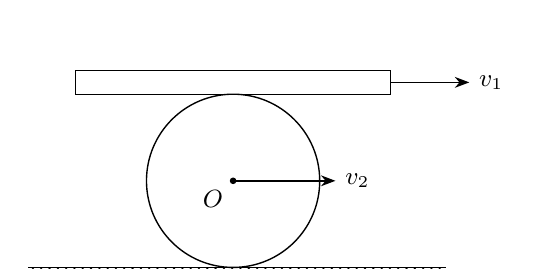
\begin{tikzpicture}[x=1cm,y=1cm,line width=0.5pt,>=Stealth,font=\small]
\draw[fill=white] (0.3,2.2) rectangle (4.3,2.5); \draw[->] (4.3,2.35)--(5.3,2.35) node[right]{$v_1$};
\draw (2.3,1.1) circle(1.1); \fill (2.3,1.1) circle(1.2pt); \node[below left] at (2.3,1.1) {$O$}; \draw[->] (2.3,1.1)--(3.6,1.1) node[right]{$v_2$};
\draw (-0.3,0)--(5.0,0); \fill[pattern=north east lines,draw=none] (-0.3,-0.15) rectangle (5.0,0);
\end{tikzpicture}\par\smallskip
\opt{A}{5}
\opt{B}{2,5}
\opt{C}{10}
\opt{D}{7,5}
\end{minipage}\vspace{2pt}\par
\noindent\colorbox{gray!12}{\parbox{\dimexpr\linewidth-2\fboxsep}{\textbf{Javob: A) 5}}}\par\smallskip
\noindent\textit{Yechim.}\ Tanga sirpanmasdan dumalaydi: pastki nuqta tezligi nol, yuqorigi nuqta tezligi $v_1$ (çizğiç bilan birga). Markaz tezligi ikki marta kiçik: $v_2=v_1/2=5$ cm/s.\par\par\medskip\hrule\medskip
\Needspace{10\baselineskip}\noindent\begin{minipage}{\linewidth}
\textbf{7.}\ Koordinata boşidan 5 m/s tezlikda yölga çiqqan jism 6 s harakatlanib neçançi koordinataga (m) boradi?\par\smallskip
\opt{A}{30}
\opt{B}{15}
\opt{C}{10}
\opt{D}{20}
\end{minipage}\vspace{2pt}\par
\noindent\colorbox{gray!12}{\parbox{\dimexpr\linewidth-2\fboxsep}{\textbf{Javob: A) 30}}}\par\smallskip
\noindent\textit{Yechim.}\ $x=vt=5\cdot6=30$ m.\par\par\medskip\hrule\medskip
\Needspace{10\baselineskip}\noindent\begin{minipage}{\linewidth}
\textbf{8.}\ $m$ massali, $l$ uzunlikdagi sterjen tik holda suvda suzib yuribdi, uning suvning içidagi qismi 0,8$l$. Sterjenni tik holda suvdan çiqariş uçun zarur bölgan minimal energiya hisoblansin.\par\smallskip
\opt{A}{$0{,}4mgl$}
\opt{B}{$0{,}8mgl$}
\opt{C}{$0{,}35mgl$}
\opt{D}{$0{,}25mgl$}
\end{minipage}\vspace{2pt}\par
\noindent\colorbox{gray!12}{\parbox{\dimexpr\linewidth-2\fboxsep}{\textbf{Javob: A) $0{,}4mgl$}}}\par\smallskip
\noindent\textit{Yechim.}\ Suziş şarti $m=\rho_s S\cdot0{,}8l$. Sterjen $y$ ga kötarilganda zarur kuç $F=mg-\rho_s gS(0{,}8l-y)=\rho_s gSy$ (muvozanatda $F=0$). $y$ $0$ dan $0{,}8l$ gaça:\par
\[A=\frac{\rho_s gS(0{,}8l)^2}{2}=0{,}32\,\rho_s gSl^2=0{,}32\,gl\cdot\frac{m}{0{,}8}=0{,}4mgl.\]\par\medskip\hrule\medskip
\Needspace{10\baselineskip}\noindent\begin{minipage}{\linewidth}
\textbf{9.}\ Quyidagi grafikda jism tezligining köçişiga boğliqlik grafigi keltirilgan. Jismning tezlanişini (m/s$^{2}$) aniqlang.\par\smallskip
\noindent\hspace*{4mm}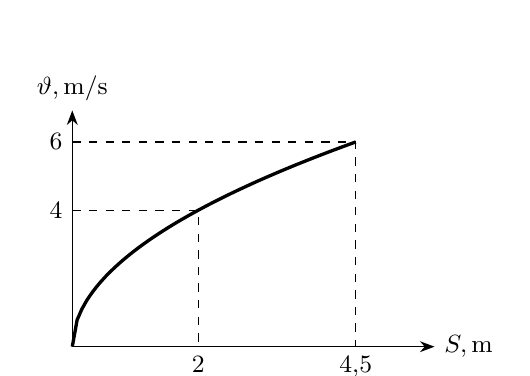
\begin{tikzpicture}[x=1cm,y=1cm,line width=0.5pt,>=Stealth,font=\small]
\draw[->] (0,0)--(4.6,0) node[right]{$S,\mathrm{m}$}; \draw[->] (0,0)--(0,3.0) node[above]{$\vartheta,\mathrm{m/s}$};
\draw[very thick,domain=0:3.6,samples=60] plot (\x,{0.43333*sqrt(10*\x)});
\draw[dashed] (0,1.733)--(1.6,1.733)--(1.6,0) (0,2.6)--(3.6,2.6)--(3.6,0);
\node[left] at (0,1.733) {$4$}; \node[left] at (0,2.6) {$6$}; \node[below] at (1.6,0) {$2$}; \node[below] at (3.6,0) {$4{,}5$};
\end{tikzpicture}\par\smallskip
\opt{A}{40}
\opt{B}{2}
\opt{C}{100}
\opt{D}{4}
\end{minipage}\vspace{2pt}\par
\noindent\colorbox{gray!12}{\parbox{\dimexpr\linewidth-2\fboxsep}{\textbf{Javob: D) 4}}}\par\smallskip
\noindent\textit{Yechim.}\ Grafikdan: $S_1=2$ m da $v_1=4$ m/s, $S_2=4{,}5$ m da $v_2=6$ m/s. $v_2^2-v_1^2=2a(S_2-S_1)$:\par
\[a=\frac{36-16}{2\cdot2{,}5}=4\ \text{m/s}^2.\]\par\medskip\hrule\medskip
\Needspace{10\baselineskip}\noindent\begin{minipage}{\linewidth}
\textbf{10.}\ Quyida ifodalangan qonunni qanday nomlasa böladi? Agar jism bir neça kuç ta’sirida harakatlanayotgan bölsa, har bir kuç boşqa kuçlar bilan birgalikda yoki yakka ö ta’sir qilayotganidan qat’iy nazar jismga hamma vaqt bir xil tezlaniş beradi.\par\smallskip
\opt{A}{kuçlar ta’sirining mustaqillik qonuni}
\opt{B}{inersiya qonuni}
\opt{C}{impulsning saqlaniş qonuni}
\opt{D}{Nyutonning II qonuni}
\end{minipage}\vspace{2pt}\par
\noindent\colorbox{gray!12}{\parbox{\dimexpr\linewidth-2\fboxsep}{\textbf{Javob: A) kuçlar ta’sirining mustaqillik qonuni}}}\par\smallskip
\noindent\textit{Yechim.}\ Bu kuçlar ta’sirining mustaqillik qonuni (superpozitsiya prinsipi).\par\par\medskip\hrule\medskip
\Needspace{10\baselineskip}\noindent\begin{minipage}{\linewidth}
\textbf{11.}\ Ideal gazning absolyut temperaturasi 2 marta ortganda uning bosimi 50 \% ga ortdi. Gazning hajmi neça marta özgargan?\par\smallskip
\opt{A}{4/3 marta kamaygan}
\opt{B}{5/3 marta ortgan}
\opt{C}{5/3 marta kamaygan}
\opt{D}{4/3 marta ortgan}
\end{minipage}\vspace{2pt}\par
\noindent\colorbox{gray!12}{\parbox{\dimexpr\linewidth-2\fboxsep}{\textbf{Javob: D) 4/3 marta ortgan}}}\par\smallskip
\noindent\textit{Yechim.}\ $\frac{pV}{T}=\text{const}$: $V_2=V_1\frac{p_1T_2}{p_2T_1}=V_1\cdot\frac{2}{1{,}5}=\frac43V_1$ — hajm $4/3$ marta ortgan.\par\par\medskip\hrule\medskip
\Needspace{10\baselineskip}\noindent\begin{minipage}{\linewidth}
\textbf{12.}\ Hajmlari 100 l va 250 l bölgan ikkita idişda bir xil temperaturali havo bor. Birinçisidagi havoning nisbiy namligi 25 \%. Idişlar birlaştirilgaç havoning nisbiy namligi 35 \% bölib qoldi. Ikkinçi idişdagi havoning nisbiy namligi (\%) dastlab qanday bölgan? (Jarayon izotermik)\par\smallskip
\opt{A}{10}
\opt{B}{39}
\opt{C}{60}
\opt{D}{50}
\end{minipage}\vspace{2pt}\par
\noindent\colorbox{gray!12}{\parbox{\dimexpr\linewidth-2\fboxsep}{\textbf{Javob: B) 39}}}\par\smallskip
\noindent\textit{Yechim.}\ Izotermik jarayonda buğ massasi $\varphi V$ ga proporsional va saqlanadi:\par
\[25\cdot100+\varphi_2\cdot250=35\cdot350\ \Rightarrow\ \varphi_2=\frac{12\,250-2500}{250}=39\%.\]\par\medskip\hrule\medskip
\Needspace{10\baselineskip}\noindent\begin{minipage}{\linewidth}
\textbf{13.}\ 1,204$\cdot10^{24}$ ta molekuladan tarkib topgan gazning modda miqdorini toping (mol). NA =6,02$\cdot10^{23}$ mol$-$1.\par\smallskip
\opt{A}{0,2}
\opt{B}{20}
\opt{C}{2}
\opt{D}{200}
\end{minipage}\vspace{2pt}\par
\noindent\colorbox{gray!12}{\parbox{\dimexpr\linewidth-2\fboxsep}{\textbf{Javob: C) 2}}}\par\smallskip
\noindent\textit{Yechim.}\ $\nu=N/N_A=1{,}204\cdot10^{24}/6{,}02\cdot10^{23}=2$ mol.\par\par\medskip\hrule\medskip
\Needspace{10\baselineskip}\noindent\begin{minipage}{\linewidth}
\textbf{14.}\ Yuzasi 1 m$^{2}$ bölgan silindrda 200 N oğirlikdagi erkin siljiy oladigan porşen bor. Agar gaz hajmi 10 l ga kamaysa, taşqi kuçlarning bajargan işini toping (J). Taşqi atmosfera bosimini hisobga olmang.\par\smallskip
\opt{A}{1}
\opt{B}{3}
\opt{C}{2}
\opt{D}{4}
\end{minipage}\vspace{2pt}\par
\noindent\colorbox{gray!12}{\parbox{\dimexpr\linewidth-2\fboxsep}{\textbf{Javob: C) 2}}}\par\smallskip
\noindent\textit{Yechim.}\ Gaz bosimi $p=P/S=200$ Pa. Taşqi kuçlar işi $A=p\Delta V=200\cdot0{,}01=2$ J.\par\par\medskip\hrule\medskip
\Needspace{10\baselineskip}\noindent\begin{minipage}{\linewidth}
\textbf{15.}\ Massalari örtaça 17,4 $\mu$g dan bölgan çang zarralari havoda uçib yuribdi. Agar havoning molyar massasi 29 g/mol ga teng bölsa, çang zarralari va havo molekulalarining örtaça kvadratik tezliklarini taqqoslang. NA =6$\cdot10^{23}$ mol$-$1.\par\smallskip
\opt{A}{çang zarralari tezligi 600 mln marta katta}
\opt{B}{havo molekulalari tezligi 600 mln marta katta}
\opt{C}{havo molekulalari tezligi 100 mln marta katta}
\opt{D}{bir xil}
\end{minipage}\vspace{2pt}\par
\noindent\colorbox{gray!12}{\parbox{\dimexpr\linewidth-2\fboxsep}{\textbf{Javob: B) havo molekulalari tezligi 600 mln marta katta}}}\par\smallskip
\noindent\textit{Yechim.}\ Bir xil temperaturada $\frac{mv^2}{2}$ bir xil, ya’ni $v\sim1/\sqrt m$. Havo molekulasi massasi $m_0=\frac{0{,}029}{6\cdot10^{23}}\approx4{,}83\cdot10^{-26}$ kg, çang zarrasi $1{,}74\cdot10^{-8}$ kg.\par
\[\frac{v_h}{v_{ch}}=\sqrt{\frac{1{,}74\cdot10^{-8}}{4{,}83\cdot10^{-26}}}=\sqrt{3{,}6\cdot10^{17}}=6\cdot10^8.\]
Havo molekulalari tezligi 600 mln marta katta.\par\par\medskip\hrule\medskip
\Needspace{10\baselineskip}\noindent\begin{minipage}{\linewidth}
\textbf{16.}\ Akkumulyator EYuK 12 V, töplagan zaryadi 60 A$\cdot$h. Uning içki qarşiligi 0,5 $\Omega$, taşqi zanjir qarşiligi 11,5 $\Omega$ bölsa, akkumulyator taşqi zanjirga qança energiya (kJ) bera oladi?\par\smallskip
\opt{A}{2376}
\opt{B}{2484}
\opt{C}{1980}
\opt{D}{2070}
\end{minipage}\vspace{2pt}\par
\noindent\colorbox{gray!12}{\parbox{\dimexpr\linewidth-2\fboxsep}{\textbf{Javob: B) 2484}}}\par\smallskip
\noindent\textit{Yechim.}\ $I=\frac{\mathcal E}{R+r}=1$ A, taşqi kuçlaniş $U=IR=11{,}5$ V. Zaryad $q=60\cdot3600=216\,000$ C:\par
\[W=qU=216\,000\cdot11{,}5=2{,}484\cdot10^6\ \text{J}=2484\ \text{kJ}.\]\par\medskip\hrule\medskip
\Needspace{10\baselineskip}\noindent\begin{minipage}{\linewidth}
\textbf{17.}\ E.Yu.K $E$, içki qarşiligi $r$ bölgan $n$ ta tok manbai özaro ketma-ket ulandi va batareya hosil qilindi. Agar batareyaga $R$ taşqi qarşilik ulansa, zanjirdagi tok kuçi qanday böladi? $R\gg n\cdot r$.\par\smallskip
\opt{A}{$\approx\dfrac{E}{R}$}
\opt{B}{$\approx\dfrac{E}{nR}$}
\opt{C}{$\approx\dfrac{nE}{R}$}
\opt{D}{$\approx\dfrac{E}{nr}$}
\end{minipage}\vspace{2pt}\par
\noindent\colorbox{gray!12}{\parbox{\dimexpr\linewidth-2\fboxsep}{\textbf{Javob: C) $\approx\dfrac{nE}{R}$}}}\par\smallskip
\noindent\textit{Yechim.}\ $I=\frac{nE}{R+nr}\approx\frac{nE}{R}$, çunki $R\gg nr$.\par\par\medskip\hrule\medskip
\Needspace{10\baselineskip}\noindent\begin{minipage}{\linewidth}
\textbf{18.}\ Qarşiligi 2 $\Omega$ dan bölgan 6 ta ötkazgiç juftlab parallel ulandi. Uçala juft öz navbatida içki qarşiligi 1 $\Omega$ bölgan batareyaga ketma-ket ulandi. Bunda har bir ötkazgiçdan 2,5 A tok ötdi. Agar ulardan biri uzilsa, zanjirdagi tok kuçi qanday böladi (A)?\par\smallskip
\opt{A}{1}
\opt{B}{2}
\opt{C}{4}
\opt{D}{6}
\end{minipage}\vspace{2pt}\par
\noindent\colorbox{gray!12}{\parbox{\dimexpr\linewidth-2\fboxsep}{\textbf{Javob: C) 4}}}\par\smallskip
\noindent\textit{Yechim.}\ Har bir juft qarşiligi $1\ \Omega$, taşqi zanjir $3\ \Omega$; har bir juftdan $2\cdot2{,}5=5$ A ötadi. $\mathcal E=5(3+1)=20$ V. Bitta ötkazgiç uzilsa, taşqi qarşilik $1+1+2=4\ \Omega$:\par
\[I=\frac{20}{4+1}=4\ \text{A}.\]\par\medskip\hrule\medskip
\Needspace{10\baselineskip}\noindent\begin{minipage}{\linewidth}
\textbf{19.}\ Ikki musbat zaryadlardan birining miqdori 3 marta orttirilsa, ular orasidagi ta’sir kuçi qanday özgaradi?\par\smallskip
\opt{A}{3 marta ortadi}
\opt{B}{3 marta kamayadi}
\opt{C}{özgarmaydi}
\opt{D}{9 marta ortadi}
\end{minipage}\vspace{2pt}\par
\noindent\colorbox{gray!12}{\parbox{\dimexpr\linewidth-2\fboxsep}{\textbf{Javob: A) 3 marta ortadi}}}\par\smallskip
\noindent\textit{Yechim.}\ $F=k\frac{q_1q_2}{r^2}\sim q_1$ — kuç 3 marta ortadi.\par\par\medskip\hrule\medskip
\Needspace{10\baselineskip}\noindent\begin{minipage}{\linewidth}
\textbf{20.}\ Tebraniş konturi induktivligi 0,5 H bölgan ğaltak va siğimi 20 mF bölgan kondensatordan iborat. Agar kondensatordagi kuçlaniş 2 V bölgan paytda ğaltakdagi tok kuçi 0,3 A bölgan bölsa, konturdagi tok kuçining maksimal qiymatini (A) aniqlang.\par\smallskip
\opt{A}{0,4}
\opt{B}{0,5}
\opt{C}{0,6}
\opt{D}{0,8}
\end{minipage}\vspace{2pt}\par
\noindent\colorbox{gray!12}{\parbox{\dimexpr\linewidth-2\fboxsep}{\textbf{Javob: B) 0,5}}}\par\smallskip
\noindent\textit{Yechim.}\ Konturda töliq energiya saqlanadi:\par
\[\frac{LI_0^2}{2}=\frac{LI^2}{2}+\frac{CU^2}{2}\ \Rightarrow\ I_0^2=0{,}09+\frac{0{,}02\cdot4}{0{,}5}=0{,}25,\quad I_0=0{,}5\ \text{A}.\]\par\medskip\hrule\medskip
\Needspace{10\baselineskip}\noindent\begin{minipage}{\linewidth}
\textbf{21.}\ Qarşiliklari $R_1$ = 6 $\Omega$ va $R_2$ = 12 $\Omega$ bölgan ötkazgiçlar $U$ = 36 V tok manbayiga ketma-ket ulandi. $R_2$ qarşilikdagi kuçlanişni (V) toping.\par\smallskip
\opt{A}{12}
\opt{B}{18}
\opt{C}{24}
\opt{D}{6}
\end{minipage}\vspace{2pt}\par
\noindent\colorbox{gray!12}{\parbox{\dimexpr\linewidth-2\fboxsep}{\textbf{Javob: C) 24}}}\par\smallskip
\noindent\textit{Yechim.}\ $I=\frac{36}{18}=2$ A, $U_2=IR_2=24$ V.\par\par\medskip\hrule\medskip
\Needspace{10\baselineskip}\noindent\begin{minipage}{\linewidth}
\textbf{22.}\ Özgaruvçan tok manbayiga induktivligi 25 mH bölgan ğaltak ulangan. Agar zanjirdagi tok $i = 4\cos(100\pi t)$ [A] qonun bilan özgarsa, ğaltak uçlaridagi kuçlaniş qanday qonun bilan özgarişini (V) aniqlang.\par\smallskip
\opt{A}{$u = 10\pi\cos(100\pi t + \dfrac{\pi}{2})$}
\opt{B}{$u = 10\pi\cos(100\pi t)$}
\opt{C}{$u = 10\pi\cos(100\pi t - \dfrac{\pi}{2})$}
\opt{D}{$u = -10\pi\cos(100\pi t)$}
\end{minipage}\vspace{2pt}\par
\noindent\colorbox{gray!12}{\parbox{\dimexpr\linewidth-2\fboxsep}{\textbf{Javob: A) $u = 10\pi\cos(100\pi t + \dfrac{\pi}{2})$}}}\par\smallskip
\noindent\textit{Yechim.}\ $U_0=\omega LI_0=100\pi\cdot0{,}025\cdot4=10\pi$ V. Ğaltakda kuçlaniş tokdan faza böyiça $\pi/2$ ga oldinda: $u=10\pi\cos(100\pi t+\pi/2)$.\par\par\medskip\hrule\medskip
\Needspace{10\baselineskip}\noindent\begin{minipage}{\linewidth}
\textbf{23.}\ Texnik qöllanmalarda galvanostegiyaning qöllanilişiga doir ma’lumotda h/ kattalik keltiriladi. Bu kattalik nimani ifodalaydi? 1) birlik tok ziçligida qoplaş qalinligining ortiş tezligi; 2) metall elektrokimyoviy ekvivalentini uning ziçligiga nisbati; 3) sarf böladigan energiya miqdori.\par\smallskip
\opt{A}{3}
\opt{B}{2,3}
\opt{C}{1,3}
\opt{D}{1,2}
\end{minipage}\vspace{2pt}\par
\noindent\colorbox{gray!12}{\parbox{\dimexpr\linewidth-2\fboxsep}{\textbf{Javob: D) 1,2}}}\par\smallskip
\noindent\textit{Yechim.}\ Qoplama massasi $m=\rho hS=kjSt$, bundan $\frac{h}{jt}=\frac{k}{\rho}$. Bu birlik tok ziçligida qatlam qalinligining ortiş tezligi (1) va elektrokimyoviy ekvivalentning ziçlikka nisbati (2).\par\par\medskip\hrule\medskip
\Needspace{10\baselineskip}\noindent\begin{minipage}{\linewidth}
\textbf{24.}\ Zaryadlangan jism atrofidagi elektr maydon kuç çiziqlari jism sirtiga nisbatan qanday joylaşadi?\par\smallskip
\opt{A}{parallel}
\opt{B}{tik}
\opt{C}{qiya}
\opt{D}{ixtiyoriy}
\end{minipage}\vspace{2pt}\par
\noindent\colorbox{gray!12}{\parbox{\dimexpr\linewidth-2\fboxsep}{\textbf{Javob: B) tik}}}\par\smallskip
\noindent\textit{Yechim.}\ Ötkazgiç sirti ekvipotensial, maydon kuç çiziqlari unga tik.\par\par\medskip\hrule\medskip
\Needspace{10\baselineskip}\noindent\begin{minipage}{\linewidth}
\textbf{25.}\ E.Yu.K $\varepsilon$ bölgan tok manbai taşqi zanjirga ulanmagan. Mazkur holatda manba qutblaridagi $U$ kuçlanişni toping.\par\smallskip
\opt{A}{$U=\varepsilon$}
\opt{B}{0}
\opt{C}{$U<\varepsilon$}
\opt{D}{$U>\varepsilon$}
\end{minipage}\vspace{2pt}\par
\noindent\colorbox{gray!12}{\parbox{\dimexpr\linewidth-2\fboxsep}{\textbf{Javob: A) $U=\varepsilon$}}}\par\smallskip
\noindent\textit{Yechim.}\ Zanjir oçiq, tok yöq, içki qarşilikda kuçlaniş tuşmaydi: $U=\varepsilon$.\par\par\medskip\hrule\medskip
\Needspace{10\baselineskip}\noindent\begin{minipage}{\linewidth}
\textbf{26.}\ Optik kuçi 6 dptr bölgan yiğuvçi linza yordamida ekranda buyumning 2 marta kiçiklaşgan haqiqiy tasviri hosil qilindi. Buyum va tasvir orasidagi masofani (m) aniqlang\par\smallskip
\opt{A}{1/2}
\opt{B}{3/4}
\opt{C}{2}
\opt{D}{1/4}
\end{minipage}\vspace{2pt}\par
\noindent\colorbox{gray!12}{\parbox{\dimexpr\linewidth-2\fboxsep}{\textbf{Javob: B) 3/4}}}\par\smallskip
\noindent\textit{Yechim.}\ $F=1/6$ m. $\Gamma=1/2$: $d=F(1+2)=0{,}5$ m, $f=0{,}25$ m. Masofa $d+f=0{,}75=3/4$ m.\par\par\medskip\hrule\medskip
\Needspace{10\baselineskip}\noindent\begin{minipage}{\linewidth}
\textbf{27.}\ Yiğuvçi linzadan buyumgaça masofa 10 cm ga teng. Linzada buyumning 2 marta kattalaşgan mavhum tasviri hosil bölgan bölsa, uning fokus masofasini (cm) aniqlang.\par\smallskip
\opt{A}{5}
\opt{B}{20}
\opt{C}{50}
\opt{D}{100}
\end{minipage}\vspace{2pt}\par
\noindent\colorbox{gray!12}{\parbox{\dimexpr\linewidth-2\fboxsep}{\textbf{Javob: B) 20}}}\par\smallskip
\noindent\textit{Yechim.}\ Mavhum tasvir: $f=-2d=-20$ cm. $\frac1F=\frac1{10}-\frac1{20}=\frac1{20}$, $F=20$ cm.\par\par\medskip\hrule\medskip
\Needspace{10\baselineskip}\noindent\begin{minipage}{\linewidth}
\textbf{28.}\ Fokus masofasi 15 cm bölgan linzada buyumning 3 marta kiçiklaşgan teskari tasviri hosil böldi. Buyumdan tasvirgaça bölgan masofani (cm) aniqlang.\par\smallskip
\opt{A}{80}
\opt{B}{60}
\opt{C}{45}
\opt{D}{90}
\end{minipage}\vspace{2pt}\par
\noindent\colorbox{gray!12}{\parbox{\dimexpr\linewidth-2\fboxsep}{\textbf{Javob: A) 80}}}\par\smallskip
\noindent\textit{Yechim.}\ $\Gamma=1/3$: $d=F(1+3)=60$ cm, $f=d/3=20$ cm. Masofa $60+20=80$ cm.\par\par\medskip\hrule\medskip
\Needspace{10\baselineskip}\noindent\begin{minipage}{\linewidth}
\textbf{29.}\ Metall sirtiga tuşayotgan fotonning töliq energiyasi 3 eV ga, sirtdan ajralayotgan fotoelektronlarning maksimal kinetik energiyasi esa 2 eV ga teng. Agar fotonning çastotasi 3 marta orttirilsa, fotoelektronlarning maksimal kinetik energiyasi neça marta ortadi?\par\smallskip
\opt{A}{10}
\opt{B}{2}
\opt{C}{4}
\opt{D}{20}
\end{minipage}\vspace{2pt}\par
\noindent\colorbox{gray!12}{\parbox{\dimexpr\linewidth-2\fboxsep}{\textbf{Javob: C) 4}}}\par\smallskip
\noindent\textit{Yechim.}\ Çiqiş işi $A=3-2=1$ eV. Çastota 3 marta ortsa $\varepsilon=9$ eV, $E_k=9-1=8$ eV — 4 marta ortadi.\par\par\medskip\hrule\medskip
\Needspace{10\baselineskip}\noindent\begin{minipage}{\linewidth}
\textbf{30.}\ Proton elektr maydonida 6,4$\cdot10^{11}$ m/s$^{2}$ tezlaniş bilan harakatlanişi uçun elektr maydon kuçlanganligi qanday (kV/m) bölişi kerak?\par\smallskip
\opt{A}{6,64}
\opt{B}{3,32}
\opt{C}{13,28}
\opt{D}{11,72}
\end{minipage}\vspace{2pt}\par
\noindent\colorbox{gray!12}{\parbox{\dimexpr\linewidth-2\fboxsep}{\textbf{Javob: A) 6,64}}}\par\smallskip
\noindent\textit{Yechim.}\ \[E=\frac{ma}{e}=\frac{1{,}66\cdot10^{-27}\cdot6{,}4\cdot10^{11}}{1{,}6\cdot10^{-19}}\approx6{,}64\cdot10^3\ \text{V/m}=6{,}64\ \text{kV/m}.\]\par\medskip\hrule\medskip
\Needspace{10\baselineskip}\noindent\begin{minipage}{\linewidth}
\textbf{31.}\ Yoruğlik tezligiga yaqin tezlikda harakatlanayotgan zarraçaning impulsini tinçlikdagi energiyasiga nisbati $P/E_0=1{,}5/c$ ga teng. Zarraça töliq energiyasini uning tinçlikdagi energiyasiga nisbati $E_T/E_0$ ni toping. $c$ - yoruglikning böşliqdagi tezligi.\par\smallskip
\opt{A}{$\approx1{,}8$}
\opt{B}{$\approx2$}
\opt{C}{$\approx2{,}1$}
\opt{D}{$\approx1{,}2$}
\end{minipage}\vspace{2pt}\par
\noindent\colorbox{gray!12}{\parbox{\dimexpr\linewidth-2\fboxsep}{\textbf{Javob: A) $\approx1{,}8$}}}\par\smallskip
\noindent\textit{Yechim.}\ $E^2=E_0^2+p^2c^2$:\par
\[\frac{E}{E_0}=\sqrt{1+\left(\frac{pc}{E_0}\right)^2}=\sqrt{1+2{,}25}\approx1{,}8.\]\par\medskip\hrule\medskip
\Needspace{10\baselineskip}\noindent\begin{minipage}{\linewidth}
\textbf{32.}\ 32 kg massali jism 400 N kuç bilan tik yuqoriga kötarilmoqda. Jism 42 m balandlikka kötarilganda kuçning bajargan işi (J) nimaga teng?\par\smallskip
\opt{A}{16800}
\opt{B}{13440}
\opt{C}{14400}
\opt{D}{18200}
\end{minipage}\vspace{2pt}\par
\noindent\colorbox{gray!12}{\parbox{\dimexpr\linewidth-2\fboxsep}{\textbf{Javob: A) 16800}}}\par\smallskip
\noindent\textit{Yechim.}\ $A=Fh=400\cdot42=16\,800$ J.\par\par\medskip\hrule\medskip
\newpage\noindent\textbf{33–35.}\ Vakuumda bir-biridan 6 cm masofada turgan $q=+4$ nC va $-q$ zaryadlar orasidagi kesmaning örtasida $A$ nuqta joylaşgan (rasm). $k=9\cdot10^9\ \mathrm{N\cdot m^2/C^2}$.\par\medskip
\begin{center}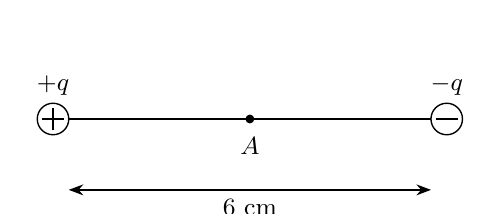
\begin{tikzpicture}[x=1cm,y=1cm,line width=0.5pt,>=Stealth,font=\small]
\draw (0,0)--(5.0,0); \foreach \x/\n in {0/{+q},5.0/{-q}}{\draw[fill=white] (\x,0) circle(0.2); \node[above=5pt] at (\x,0) {$\n$};}
\draw (-0.14,0)--(0.14,0) (0,-0.14)--(0,0.14); \draw (4.86,0)--(5.14,0);
\fill (2.5,0) circle(1.6pt) node[below=3pt]{$A$}; \draw[<->] (0.2,-0.9)--(4.8,-0.9); \node[below] at (2.5,-0.9) {$6\ \mathrm{cm}$};
\end{tikzpicture}\end{center}
\noindent\textbf{33.}\ $A$ nuqtadagi elektr maydon kuçlanganligini (kV/m) toping.\par
\noindent\textbf{34.}\ $A$ nuqtadagi maydon potensialini (V) toping.\par
\noindent\textbf{35.}\ $A$ nuqtaga qöyilgan $2$ nC zaryadga ta’sir qiluvçi kuçni ($\mu$N) toping.\par
\noindent Variantlar: A) 0;\quad B) 20;\quad C) 40;\quad D) 80;\quad E) 160;\quad F) 320\par\smallskip
\noindent\colorbox{gray!12}{\parbox{\dimexpr\linewidth-2\fboxsep}{\textbf{Javob: 33--D) 80; 34--A) 0; 35--E) 160}}}\par\smallskip
\noindent\textit{Yechim.}\ Örta nuqtada ikkala zaryadning maydoni bir tomonga ($+q$ dan $-q$ ga) yönalgan, har biri $r=3$ cm masofada:\par
\[E=2\frac{kq}{r^2}=2\cdot\frac{9\cdot10^9\cdot4\cdot10^{-9}}{9\cdot10^{-4}}=8\cdot10^4\ \text{V/m}=80\ \text{kV/m}.\]
Potensial $\varphi=\frac{kq}{r}-\frac{kq}{r}=0$. Kuç $F=q'E=2\cdot10^{-9}\cdot8\cdot10^4=1{,}6\cdot10^{-4}$ N $=160\ \mu$N.\par\par\medskip\hrule\medskip
\Needspace{12\baselineskip}\noindent\textbf{36.}\ Massasi 2 kg bölgan brusok qiyalik burçagi $37^\circ$ bölgan silliq qiya tekislikda bikrligi 200 N/m bölgan prujina yordamida muvozanatda uşlab turilibdi (prujina qiya tekislikka parallel). $\sin37^\circ=0{,}6$, $g=10$ m/s$^2$.\par
\noindent\hspace*{4mm}a)\ Prujinaning çözilişini (cm) toping.\par
\noindent\hspace*{4mm}b)\ Qiya tekislikning brusokka ta’sir qiluvçi normal reaksiya kuçini (N) toping.\par
\noindent\colorbox{gray!12}{\parbox{\dimexpr\linewidth-2\fboxsep}{\textbf{Javob: a)\ 6;\quad b)\ 16}}}\par\smallskip
\noindent\textit{Yechim.}\ Tekislik böylab: $kx=mg\sin37^\circ=12$ N, $x=12/200=0{,}06$ m $=6$ cm. Normal reaksiya $N=mg\cos37^\circ=20\cdot0{,}8=16$ N.\par\par\medskip\hrule\medskip
\Needspace{12\baselineskip}\noindent\textbf{37.}\ 20 m balandlikdan gorizontal otilgan jism Yerga gorizontga $45^\circ$ burçak ostida urildi. Havoning qarşiligi hisobga olinmasin, $g=10$ m/s$^2$.\par
\noindent\hspace*{4mm}a)\ Jismning boşlanğiç tezligini (m/s) toping.\par
\noindent\hspace*{4mm}b)\ Jismning gorizontal uçiş uzoqligini (m) toping.\par
\noindent\colorbox{gray!12}{\parbox{\dimexpr\linewidth-2\fboxsep}{\textbf{Javob: a)\ 20;\quad b)\ 40}}}\par\smallskip
\noindent\textit{Yechim.}\ Yerga urilişda $v_y=\sqrt{2gh}=20$ m/s; $45^\circ$ da $v_x=v_y$, demak $v_0=20$ m/s. Uçiş vaqti $t=2$ s, uzoqlik $L=v_0t=40$ m.\par\par\medskip\hrule\medskip
\Needspace{12\baselineskip}\noindent\textbf{38.}\ Şarça silliq novdan sirpanib tuşib, radiusi 0,4 m bölgan vertikal halqa («ölik sirtmoq») böylab harakatlanadi. Şarçaning massasi 0,1 kg, $g=10$ m/s$^2$.\par
\noindent\hspace*{4mm}a)\ Şarça halqani uzilmasdan aylanib çiqişi uçun qöyib yuboriladigan eng kiçik balandlikni (m) toping.\par
\noindent\hspace*{4mm}b)\ Şarça şu balandlikdan qöyib yuborilganda halqaning eng pastki nuqtasida novga beradigan bosim kuçini (N) toping.\par
\noindent\colorbox{gray!12}{\parbox{\dimexpr\linewidth-2\fboxsep}{\textbf{Javob: a)\ 1;\quad b)\ 6}}}\par\smallskip
\noindent\textit{Yechim.}\ Halqaning eng yuqori nuqtasida uzilmaslik şarti $v^2\ge gR$. Energiya: $mgh=mg\cdot2R+\frac{mgR}{2}$, $h=2{,}5R=1$ m. Eng pastki nuqtada $v^2=2gh=20$ m$^2$/s$^2$:\par
\[N=m\left(g+\frac{v^2}{R}\right)=0{,}1\left(10+\frac{20}{0{,}4}\right)=6\ \text{N}.\]\par\medskip\hrule\medskip
\Needspace{12\baselineskip}\noindent\textbf{39.}\ Hajmi 2 L bölgan idişda 300 kPa bosimli, hajmi 4 L bölgan idişda 150 kPa bosimli bir xil gaz bor. Idişlar ingiçka nay bilan tutaştirildi, temperatura özgarmaydi.\par
\noindent\hspace*{4mm}a)\ Idişlardagi qaror topgan bosimni (kPa) toping.\par
\noindent\hspace*{4mm}b)\ Birinçi idişdagi bosim neça marta kamaydi?\par
\noindent\colorbox{gray!12}{\parbox{\dimexpr\linewidth-2\fboxsep}{\textbf{Javob: a)\ 200;\quad b)\ 1,5}}}\par\smallskip
\noindent\textit{Yechim.}\ Izotermik aralaşiş: $p_1V_1+p_2V_2=p(V_1+V_2)$:\par
\[p=\frac{300\cdot2+150\cdot4}{6}=200\ \text{kPa}.\]
Birinçi idişda bosim $300/200=1{,}5$ marta kamaydi.\par\par\medskip\hrule\medskip
\Needspace{12\baselineskip}\noindent\textbf{40.}\ 100 $^\circ$C gaça qizdirilgan 0,5 kg metall jism 20 $^\circ$C temperaturali 0,5 kg suvga tuşirildi. Qaror topgan temperatura 25 $^\circ$C. $c_{suv}=4200$ J/(kg$\cdot$K), issiqlik isroflari yöq.\par
\noindent\hspace*{4mm}a)\ Suv olgan issiqlik miqdorini (kJ) toping.\par
\noindent\hspace*{4mm}b)\ Metallning soliştirma issiqlik siğimini (J/(kg$\cdot$K)) toping.\par
\noindent\colorbox{gray!12}{\parbox{\dimexpr\linewidth-2\fboxsep}{\textbf{Javob: a)\ 10,5;\quad b)\ 280}}}\par\smallskip
\noindent\textit{Yechim.}\ $Q=4200\cdot0{,}5\cdot5=10{,}5$ kJ. Metall şunça issiqlik bergan: $c\cdot0{,}5\cdot75=10\,500$, $c=280$ J/(kg$\cdot$K).\par\par\medskip\hrule\medskip
\Needspace{12\baselineskip}\noindent\textbf{41.}\ Ideal transformatorning birlamçi çulğamida 1000 öram bölib, u 220 V kuçlanişli tarmoqqa ulangan. Ikkilamçi çulğamda 50 öram bor va unga 5,5 $\Omega$ qarşilikli iste’molçi ulangan.\par
\noindent\hspace*{4mm}a)\ Ikkilamçi çulğamdagi kuçlanişni (V) toping.\par
\noindent\hspace*{4mm}b)\ Birlamçi çulğamdagi tok kuçini (A) toping.\par
\noindent\colorbox{gray!12}{\parbox{\dimexpr\linewidth-2\fboxsep}{\textbf{Javob: a)\ 11;\quad b)\ 0,1}}}\par\smallskip
\noindent\textit{Yechim.}\ $U_2=U_1\frac{N_2}{N_1}=220\cdot\frac{50}{1000}=11$ V; $I_2=11/5{,}5=2$ A. Ideal transformator: $U_1I_1=U_2I_2$, $I_1=\frac{22}{220}=0{,}1$ A.\par\par\medskip\hrule\medskip
\Needspace{12\baselineskip}\noindent\textbf{42.}\ Kuçlanganligi 2 kV/m bölgan bir jinsli elektr maydonda $A$ va $B$ nuqtalar bitta kuç çiziğida, bir-biridan 5 cm masofada yotadi; $B$ nuqta $A$ dan maydon yönalişi böylab joylaşgan.\par
\noindent\hspace*{4mm}a)\ $A$ va $B$ nuqtalar orasidagi potensiallar farqini (V) toping.\par
\noindent\hspace*{4mm}b)\ $3\ \mu$C zaryadni $A$ dan $B$ ga köçirişda maydon bajargan işni (mJ) toping.\par
\noindent\colorbox{gray!12}{\parbox{\dimexpr\linewidth-2\fboxsep}{\textbf{Javob: a)\ 100;\quad b)\ 0,3}}}\par\smallskip
\noindent\textit{Yechim.}\ $U=Ed=2000\cdot0{,}05=100$ V ($A$ nuqta potensiali yuqori). $A=qU=3\cdot10^{-6}\cdot100=3\cdot10^{-4}$ J $=0{,}3$ mJ.\par\par\medskip\hrule\medskip
\Needspace{12\baselineskip}\noindent\textbf{43.}\ Yoruğlik qalinligi 6 cm bölgan şişa plastinkaga tik tuşmoqda. Şişaning sindiriş körsatkiçi 1,5, $c=3\cdot10^8$ m/s.\par
\noindent\hspace*{4mm}a)\ Yoruğlikning plastinkadan ötiş vaqtini (ns) toping.\par
\noindent\hspace*{4mm}b)\ Plastinkadagi optik yöl uzunligini (cm) toping.\par
\noindent\colorbox{gray!12}{\parbox{\dimexpr\linewidth-2\fboxsep}{\textbf{Javob: a)\ 0,3;\quad b)\ 9}}}\par\smallskip
\noindent\textit{Yechim.}\ $v=c/n=2\cdot10^8$ m/s; $t=\frac{d}{v}=\frac{0{,}06}{2\cdot10^8}=3\cdot10^{-10}$ s $=0{,}3$ ns. Optik yöl $L=nd=1{,}5\cdot6=9$ cm.\par\par\medskip\hrule\medskip
\Needspace{12\baselineskip}\noindent\textbf{44.}\ Buyum va ekran orasidagi masofa 90 cm. Ular orasiga yiğuvçi linza qöyilganda ekranda buyumning 2 marta kattalaşgan aniq tasviri hosil böldi.\par
\noindent\hspace*{4mm}a)\ Linzaning fokus masofasini (cm) toping.\par
\noindent\hspace*{4mm}b)\ Buyumdan linzagaça masofani (cm) toping.\par
\noindent\colorbox{gray!12}{\parbox{\dimexpr\linewidth-2\fboxsep}{\textbf{Javob: a)\ 20;\quad b)\ 30}}}\par\smallskip
\noindent\textit{Yechim.}\ $d+f=90$ cm, $f=2d$: $d=30$ cm, $f=60$ cm. $F=\frac{df}{d+f}=\frac{30\cdot60}{90}=20$ cm.\par\par\medskip\hrule\medskip
\Needspace{12\baselineskip}\noindent\textbf{45.}\ Vodorod atomi asosiy holatining energiyasi $-13{,}6$ eV, birinçi Bor orbitasi radiusi $0{,}53\cdot10^{-10}$ m.\par
\noindent\hspace*{4mm}a)\ Ikkinçi orbita radiusini ($10^{-10}$ m) toping.\par
\noindent\hspace*{4mm}b)\ Ikkinçi energetik sathdagi atomni ionlaştiriş uçun kerak bölgan energiyani (eV) toping.\par
\noindent\colorbox{gray!12}{\parbox{\dimexpr\linewidth-2\fboxsep}{\textbf{Javob: a)\ 2,12;\quad b)\ 3,4}}}\par\smallskip
\noindent\textit{Yechim.}\ $r_n=n^2r_1$: $r_2=4\cdot0{,}53\cdot10^{-10}=2{,}12\cdot10^{-10}$ m. $E_2=-13{,}6/4=-3{,}4$ eV, ionlaştiriş energiyasi $3{,}4$ eV.\par\par\medskip\hrule\medskip
\end{document}